% Author: Rishi (condensed from report/section_recurrent_matchers.md)
\section{Recurrent matchers: Siamese character RNNs}
\label{sec:rnn}

\paragraph{Model.} The recurrent matchers read each record as a sequence of \emph{characters}, so typos,
abbreviations and transliteration variants (\emph{Glyfelle}/\emph{Glyphelle}) are small edits instead of
unknown words. The input is the normalised \texttt{name | address}, cut at 100 characters, over a vocabulary
of about 250 characters. A shared (Siamese) encoder embeds characters (64 dimensions), runs a bidirectional
recurrent layer (128 units per direction), and concatenates max- and mean-pooling over time into a record
vector $u\in\mathbb{R}^{512}$. For a record vector $u$ and a candidate vector $v$, an MLP scores
$[u; v; |u-v|; u\odot v]$~\citep{mueller2016siamese}. Three variants differ only in the cell: LSTM
(0.73M parameters), GRU (0.68M) and a vanilla Elman RNN (0.58M). They are trained with binary cross-entropy
on part-A candidate pairs, whose negatives are the hard ones retrieved by blocking: 3 epochs of 600k sampled
pairs, Adam, gradient clipping at norm 1.0.

\begin{table}[h]
\centering\small
\begin{tabular}{lccccccc}
\toprule
model & val \fhalf & test \fhalf & P & R & singleton acc. & params & train min \\
\midrule
Siamese char-BiLSTM (\nb{05a}) & 0.98920 & \textbf{0.98335} & 0.9863 & 0.9846 & 0.9454 & 0.73M & 13.3 \\
Siamese char-BiGRU (\nb{05b})  & 0.98814 & 0.98197 & 0.9850 & 0.9835 & 0.9404 & 0.68M & 13.1 \\
Siamese char-BiRNN (\nb{05c})  & 0.98374 & 0.97475 & 0.9782 & 0.9789 & 0.9085 & 0.58M & 11.9 \\
\bottomrule
\end{tabular}
\caption{Recurrent matchers on the test split (one T4 GPU).}
\label{tab:rnn}
\end{table}

\paragraph{Results.} The BiLSTM reaches 0.983 test \fhalf{} in 13 minutes, about 0.01 below the fine-tuned
cross-encoders with 380$\times$ fewer parameters (Table~\ref{tab:rnn}). LSTM and GRU differ by 0.0014, which
is within seed noise for single runs. The vanilla RNN loses 0.0086 against the BiLSTM, most of all on
singletons (0.909 vs.\ 0.945).

\begin{figure}[h]
\centering
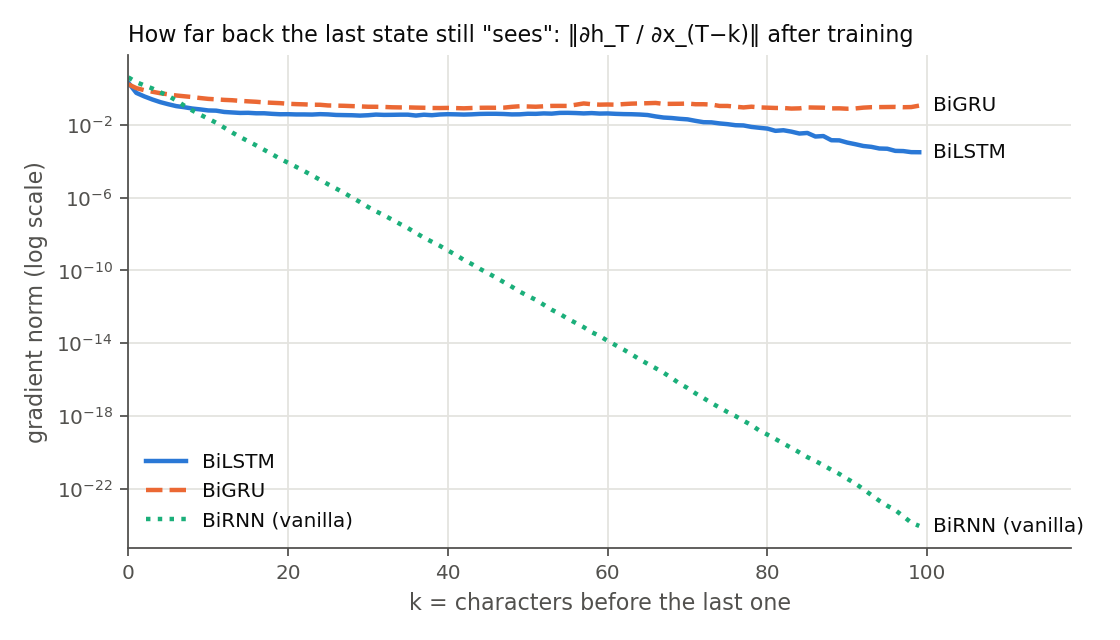
\includegraphics[width=0.72\linewidth]{rnn_grad_by_distance.png}
\caption{Gradient of the last forward state with respect to the input $k$ characters earlier, relative to
$k=0$, measured after training on 256 full-length training records.}
\label{fig:rnngrad}
\end{figure}

\paragraph{Why the vanilla RNN is worse: vanishing gradients, measured.} The vanilla RNN underfits: it has
the highest training loss at every epoch (0.044 vs.\ 0.029 for the LSTM after 3 epochs) and the largest
share of clipped steps (2.1\% in epoch 1). Figure~\ref{fig:rnngrad} measures its memory directly. For
$h_t=\tanh(Wh_{t-1}+Ux_t)$, the Jacobian $\partial h_T/\partial h_t=\prod_{s=t+1}^{T}\mathrm{diag}(1-h_s^2)\,W$
is a product of $T-t$ factors, and it shrinks geometrically~\citep{bengio1994learning,pascanu2013difficulty}:
by about 10$\times$ every 4 characters, reaching $10^{-12}$ at $k=50$. The LSTM and GRU carry state through
an additive, gated path ($\partial c_t/\partial c_{t-1}=\mathrm{diag}(f_t)$ for the LSTM), and after training
their gradient stays roughly flat over 100 characters ($2.0\times10^{-2}$ and $6.1\times10^{-2}$ at $k=50$).
At initialisation all three cells have tiny long-range gradients; only the gated cells \emph{learn} to open
the path. The gap is only about 0.01 because pooling over all time steps gives every character a short path
to the loss, and much matching evidence is local. What the vanilla RNN loses is evidence that spans the
string, such as a name token combined with a locality 60 characters later. That is what separates
near-duplicate branches, and it explains why singleton accuracy drops most.

\paragraph{Where they fail.} On the 283 records in other Indic scripts (Gujarati, Telugu, Tamil, \dots), all
three RNNs drop to 0.90--0.91, and every error is a missed link. They see only the romanised string, and
the generic romanisation of these scripts gives spellings far from the English S1 name
(\emph{emtrpraijes} for \emph{enterprises}) that the lexicon never learned (\S\ref{sec:script}).
